\documentclass[11pt, oneside]{article}  	% use "amsart" instead of "article" for AMSLaTeX format
\usepackage{geometry}                		% See geometry.pdf to learn the layout options. There are lots.
\geometry{a4paper}                   		% ... or a4paper or a5paper or ... 
%\geometry{landscape}                		% Activate for rotated page geometry
\usepackage[parfill]{parskip}    			% Activate to begin paragraphs with an empty line rather than an indent
\usepackage{graphicx}				% Use pdf, png, jpg, or eps� with pdflatex; use eps in DVI mode
								% TeX will automatically convert eps --> pdf in pdflatex		


\graphicspath{ {images/} }

\usepackage{fancyhdr}
\pagestyle{fancy}
\usepackage[latin1]{inputenc} 

% Prof. Forbes math packages
\usepackage{amsmath} % cmex10
\usepackage{amssymb}
\usepackage{amsthm}
\usepackage{bm}
\usepackage{mathrsfs}
\usepackage{wrapfig}

% Matrix command
\newcommand{\bma}[1]{\left[\begin{array}{#1}}
\newcommand{\ema}{\end{array}\right]}
\newcommand{\trans}{{\ensuremath{\mathsf{T}}}} % transpose
\newcommand{\utimes}{ {\raisebox{-0.6ex}{ \kern-1.0ex\raisebox{0.6ex}{ \small $\mathsf{v}$}}} } % 
\newcommand{\onehalf}{\mbox{$\textstyle{\frac{1}{2}}$}}


% Bold symbols
\DeclareMathAlphabet{\mbf}{OT1}{ptm}{b}{n} % for bold face Roman
\newcommand{\mbs}[1]{{\boldsymbol{#1}}} % for bold face Greek

% Other bold symbols 
\newcommand{\mbfbar}[1]{{\bar{\mbf{#1}}}}
\newcommand{\mbfhat}[1]{{\hat{\mbf{#1}}}}
\newcommand{\mbftilde}[1]{{\tilde{\mbf{#1}}}}
\newcommand{\mbsbar}[1]{{\bar{\boldsymbol{#1}}}}
\newcommand{\mbshat}[1]{{\hat{\boldsymbol{#1}}}}
\newcommand{\mbstilde}[1]{{\tilde{\boldsymbol{#1}}}}

% Physical Space, physical vectors, a vectrix, etc. 
\newcommand{\pspace}{\mathbb{P}} 
\newcommand{\ura}[1]{{\underrightarrow{{#1}}}}
\newcommand{\vectrix}[1]{\ensuremath \underrightarrow{\boldsymbol{\mathcal{F}}}_{#1}}
\def\fdota{{\raisebox{-2pt}{\LARGE $\cdot$}}}
\def\fdotb{{\raisebox{-0.6ex}{ \kern0.2ex\raisebox{0.8ex}{\tiny $\hspace*{-1ex}\circ$}}}}
\def\fddota{{\raisebox{-2pt}{\LARGE $\cdot\hspace*{-0.2ex}\cdot$}}}
\def\fddotb{{\raisebox{-0.6ex}{ \kern0.2ex\raisebox{0.8ex}{\tiny $\hspace*{-1ex}\circ\circ$}}}}
\newcommand{\fdot}[1]{{^{\fdota{\mbox{\footnotesize${#1}$}}}}}
\newcommand{\fddot}[1]{{^{\fddota{\mbox{\footnotesize${#1}$}}}}}


% Short form for equations
\newcommand{\beq}{\begin{equation}}
\newcommand{\eeq}{\end{equation}}
\newcommand{\bdis}{\begin{displaymath}}
\newcommand{\edis}{\end{displaymath}}
\newcommand{\beqarray}{\begin{eqnarray}}
\newcommand{\eeqarray}{\end{eqnarray}}
\newcommand{\beqarraynn}{\begin{eqnarray*}}
\newcommand{\eeqarraynn}{\end{eqnarray*}}

%Must be equal to ...
\newcommand{\mbeq}{\overset{!}{=}}

% Matrices shortcut
\newcommand{\crossop}[3]{\bma{ccc} 0 & -#3 & #2 \\ #3 & 0 & -#1 \\ -#2 & #1 & 0 \ema}
\newcommand{\matr}[9]{\bma{ccc} #1 & #2 & #3 \\ #4 & #5 & #6 \\ #7 & #8 & #9 \ema}
\newcommand{\colvec}[3]{\bma{c} #1 \\ #2 \\ #3 \ema}
\newcommand{\rowvec}[3]{\bma{ccc} #1 & #2 & #3 \ema}
\newcommand{\Cone}[1]{\matr{1}{0}{0}{0}{\cos(#1)}{\sin(#1)}{0}{-\sin(#1)}{\cos(#1)}}
\newcommand{\Ctwo}[1]{\matr{\cos(#1)}{0}{-\sin(#1)}{0}{1}{0}{\sin(#1)}{0}{\cos(#1)}}
\newcommand{\Cthree}[1]{\matr{\cos(#1)}{\sin(#1)}{0}{-\sin(#1)}{\cos(#1)}{0}{0}{0}{1}}

\lhead{\footnotesize MECH 642\\Advanced Dynamics}
\rhead{\footnotesize Assignment 4\\ Fr�d�ric Berdoz, 260867318} %#

\begin{document}

\title{Assignment 4} %#
\author{Fr�d�ric Berdoz\\260867318}
\date{}

\maketitle

% Question 1 ----------------------------------------------------------------------------------------------------------------------------------------------------------
\section{}
\paragraph{a)}
First,
$$\mbf{C}_{ba}=\mbf{C}_3(\theta)=\Cthree{\theta}.$$
The position of $p$ relative to $w$ is given by:
$$\ura{r}^{pw}=\vectrix{b}^\trans\mbf{r}_b^{pw}=\vectrix{a}^\trans\mbf{C}_{ba}^\trans\mbf{r}_b^{pw}=\vectrix{a}^\trans\Cthree{\theta}^\trans\colvec{x_b}{0}{0}=\vectrix{a}^\trans\underbrace{\colvec{x_b\cos(\theta)}{x_b\sin(\theta)}{0}}_{\mbf{r}_a^{pw}}$$
Thus, the velocity of $p$ relative to $w$ w.r.t. $\mathcal{F}_a$ is:
$$\ura{v}^{pw/a}={ \ura{r}^{pw} }^\fdot{a}=\left(\vectrix{a}^\trans\mbf{r}_a^{pw}\right)^\fdot{a}=\vectrix{a}^\trans\dot{\mbf{r}}_a^{pw}=\vectrix{a}^\trans\underbrace{\colvec{\dot{x}_b\cos(\theta)-x_b\sin(\theta)\dot{\theta}}{\dot{x}_b\sin(\theta)+x_b\cos(\theta)\dot{\theta}}{0}}_{\mbf{v}_a^{pw/a}}$$
Finally, the acceleration of $p$ relative to $w$ w.r.t. $\mathcal{F}_a$ is:
\begin{align*}
\ura{a}^{pw/a}& ={\ura{v}^{pw/a}}^\fdot{a}=\left(\vectrix{a}^\trans\mbf{v}_a^{pw/a}\right)^\fdot{a}=\vectrix{a}^\trans\dot{\mbf{v}}_a^{pw/a}
\\ & =\vectrix{a}^\trans\underbrace{
\colvec
{\ddot{x}_b\cos(\theta)-2\dot{x}_b\sin(\theta)\dot{\theta}-x_b\cos(\theta)\dot{\theta}^2-x_b\sin(\theta)\ddot{\theta}}
{\ddot{x}_b\sin(\theta)+2\dot{x}_b\cos(\theta)\dot{\theta}-x_b\sin(\theta)\dot{\theta}^2+x_b\cos(\theta)\ddot{\theta}}
{0}
}_{\mbf{a}_a^{pw/a}}
\\ & =
\vectrix{b}^\trans\mbf{C}_{ba}\mbf{a}_a^{pw/a}
=
\vectrix{b}^\trans\underbrace{
\colvec
{\ddot{x}_b-x_b\dot{\theta}^2}
{2\dot{x}_b\dot{\theta}+x_b\ddot{\theta}}
{0}}_{\mbf{a}_b^{pw/a}}
\end{align*}

Let $\ura{f}^{pt}=\rowvec{f_{b1}^{pt}}{f_{b2}^{pt}}{f_{b3}^{pt}}\vectrix{b}$ be the reaction force of the table, $\ura{f}^{pg}=\rowvec{0}{0}{-mg}\vectrix{b}$ the gravitational force applied on $p$ and $\ura{f}^{ps}=\rowvec{-kx_b}{0}{0}\vectrix{b}$ the spring force. Using the fact that the cut in the table is frictionless, i.e. $f_{b1}^{pt}=0$, the total force acting on $p$ becomes:
$$
\ura{f}^p=\ura{f}^{pt}+\ura{f}^{pg}+\ura{f}^{ps}=\vectrix{b}^\trans\underbrace{\colvec{-kx_b}{f_{b2}^{pt}}{f_{b3}^{pt}-mg}}_{\mbf{f}_b^p}
$$

Since $\mathcal{F}_a$ is an inertial frame and $w$ is unforced, we can use Newton's Second Law to derive the differential equation that describes the motion of $p$:
$$m\ura{a}^{pw/a}=\ura{f}^p$$
$$m\vectrix{b}^\trans \mbf{a}_b^{pw/a}=\vectrix{b}^\trans\mbf{f}_b^p$$
$$m\mbf{a}_b^{pw/a}=\mbf{f}_b^p$$
\beq m\colvec
{\ddot{x}_b-x_b\dot{\theta}^2}
{2\dot{x}_b\dot{\theta}+x_b\ddot{\theta}}
{0}
=\colvec{-kx_b}{f_{b2}^{pt}}{f_{b3}^{pt}-mg}
\label{eq:ode}
\eeq
We can see straight away that $f_{b3}^{pt}=mg$.
\paragraph{b)}
Using the fact that $\dot{\theta}$ is constant (i.e. $\ddot{\theta}=0$) and rearranging, \eqref{eq:ode} can be rewritten as follows:
\begin{align} 
\ddot{x}_b+(\frac{k}{m}-\dot{\theta}^2)x_b &=0 \label{eq:ode2}\\
2\dot{x}_b\dot{\theta}-\frac{f_{b2}^{pt}}{m}&=0
\label{eq:ode3}
\end{align}
The general solution to \eqref{eq:ode2}, knowing that $\frac{k}{m}>\dot{\theta}^2$, is given by:
\beq
x_b(t)=A\cos(\omega t) + B\sin(\omega t), \quad A,B \in \mathbb{R}, \quad \omega=\sqrt{\frac{k}{m}-\dot{\theta}^2}
\label{eq:xb}
\eeq

\paragraph{c)}
First, using the initial condition $x_b(0)=0.1$, it yields:
$$x_b(0)=A=0.1$$.
Secondly, using $\dot{x}_b(0)=0$:
$$\dot{x}_b(0)=\left[-A\omega\sin(\omega t)+ B\omega \cos(\omega t ) \right]_{t=0}=B\omega=0.$$
Therefore:
$$B=0$$
and \eqref{eq:xb} can be rewritten as follows:
\beq
x_b(t)=0.1\cos(\omega t) \, \, [\mbox{m}], \quad \omega=\sqrt{\frac{k}{m}-\dot{\theta}^2}.
\label{eq:xb2}
\eeq
Lastly,
\begin{align}
\dot{x}_b&=-0.1\omega\sin(\omega t)  \, \, [\mbox{m}/\mbox{s}],
\label{eq:dxb}
\\
\ddot{x}_b&=-0.1\omega^2\cos(\omega t) \, \, [\mbox{m}/\mbox{s}^2].
\label{eq:ddxb}
\end{align}
Using \textsc{Matlab}{}, we obtain the following plots:
\begin{figure}[h]
    \centering
        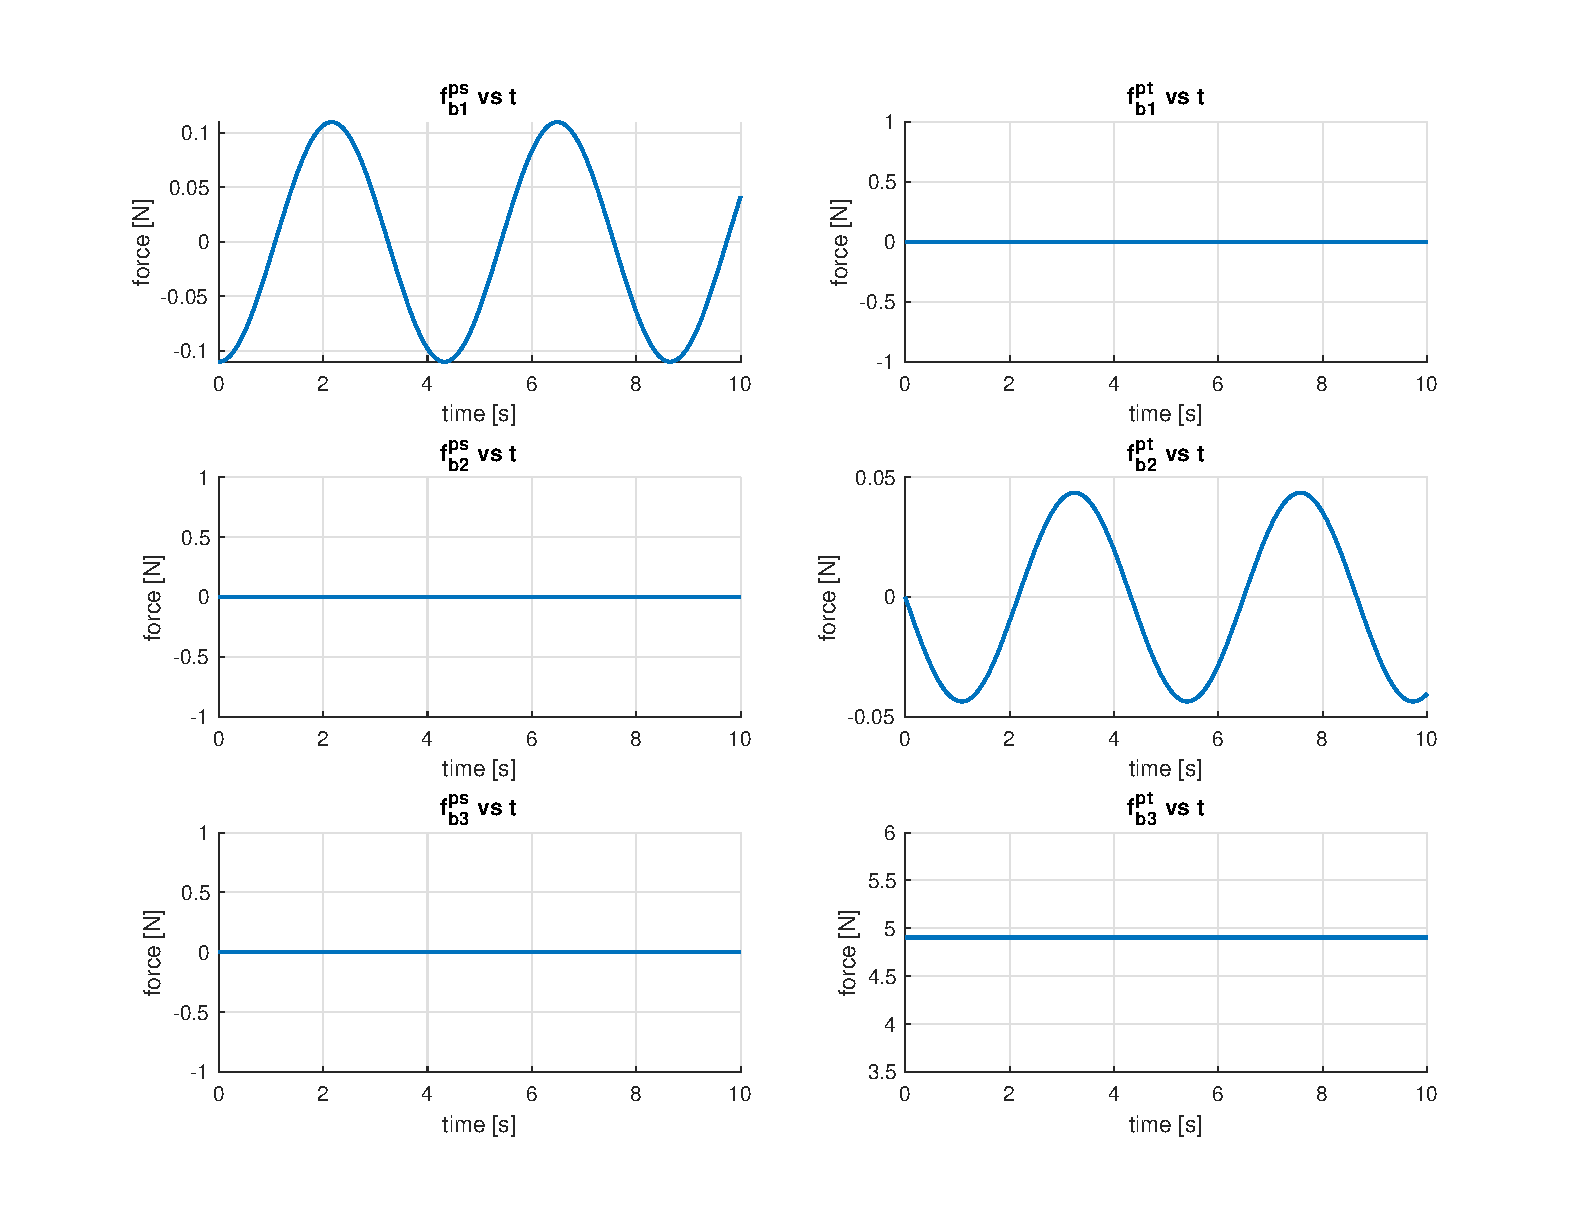
\includegraphics[width=1\textwidth]{P1c}
    \caption{$\mbf{f}_b^{pt}$ and $\mbf{f}_b^{ps}$ vs time.}
    \label{fig:P1c}
\end{figure}
\newpage
% Question 2 ----------------------------------------------------------------------------------------------------------------------------------------------------------
\section{}
\paragraph{a)}
Let $\theta$ be the angle between $\ura{b}^2$ and $\ura{a}^2$. Therefore 
\bdis
\mbf{C}_{ba}=\mbf{C}_1(\theta)=\Cone{\theta}.
\label{eq:Cba}
\edis
Moreover,
\begin{align*}
\ura{\omega}^{ba}
&=\vectrix{b}^\trans\colvec{\dot{\theta}}{0}{0},
\\ 
\\
\ura{r}^{\kappa w} 
&= \ura{r}^{\kappa c} + \ura{r}^{cw}
\\ &= \vectrix{b}^\trans\colvec{0}{y}{0}+\vectrix{b}^\trans\colvec{0}{0}{-d}
\\ &= \vectrix{b}^\trans\colvec{0}{y}{-d},
\\
\\
\ura{r}^{dmw}
&=\ura{r}^{dmc}+\ura{r}^{cw}
\\ &= \vectrix{b}^\trans \colvec{\rho_{b1}}{\rho_{b2}}{\rho_{b3}} +\vectrix{b}^\trans \colvec{0}{0}{-d}
\\ &= \vectrix{b}^\trans \colvec{\rho_{b1}}{\rho_{b2}}{\rho_{b3}-d},
\\
\\
{\ura{r}^{\kappa w}}^\fdot{a}
&={\ura{r}^{\kappa w}}^\fdot{b}+\ura{\omega}^{ba}\times{\ura{r}^{\kappa w}}
\\&=\vectrix{b}^\trans\left(\dot{\mbf{r}}_b^{\kappa w}+{\mbs{\omega}_b^{ba}}^\times\mbf{r}_b^{\kappa w}\right)
\\&=\vectrix{b}^\trans\left(\colvec{0}{\dot{y}}{0}+\matr{0}{0}{0}{0}{0}{-\dot{\theta}}{0}{\dot{\theta}}{0}\colvec{0}{y}{-d}\right)
\\&=\vectrix{b}^\trans\colvec{0}{\dot{y}+d\dot{\theta}}{y\dot{\theta}},
\end{align*}
\begin{align*}
{\ura{r}^{dmw}}^\fdot{a}
&={\ura{r}^{dm w}}^\fdot{b}+\ura{\omega}^{ba}\times{\ura{r}^{dmw}}
\\&=\vectrix{b}^\trans\left(\underbrace{\dot{\mbf{r}}_b^{dmw}}_{\mbf{=\,0}}+{\mbs{\omega}_b^{ba}}^\times\mbf{r}_b^{dm w}\right)
\\&=\vectrix{b}^\trans\left(\matr{0}{0}{0}{0}{0}{-\dot{\theta}}{0}{\dot{\theta}}{0}\colvec{\rho_{b1}}{\rho_{b2}}{\rho_{b3}-d}\right)
\\&=\vectrix{b}^\trans\colvec{0}{(d-\rho_{b3})\dot{\theta}}{\rho_{b2}\dot{\theta}}.
\end{align*}

\paragraph{b)}
Figures \ref{fig:FBDk} and \ref{fig:FBDB} show the Free Body Diagrams of the particle $\kappa$ and the body $\mathcal{B}$.
Let $\ura{f}^{r1}$ and $\ura{f}^{r1}$ be the reaction forces applied by the massless bars on the body $\mathcal{B}$.
\begin{figure}[h]
\centering
\begin{minipage}{.42\linewidth}
  \includegraphics[width=\linewidth]{FBDk}
  \caption{FBD of $\kappa$.}
  \label{fig:FBDk}
\end{minipage}
\hspace{.05\linewidth}
\begin{minipage}{.42\linewidth}
  \includegraphics[width=\linewidth]{FBDB}
  \caption{FBD of $\mathcal{B}$.}
  \label{fig:FBDB}
\end{minipage}
\end{figure}

The norm of $\ura{r}^{\kappa w}$ is 
$$\vert\vert \ura{r}^{\kappa w}\vert\vert_2={\mbf{r}_b^{\kappa w}}^\trans\mbf{r}_b^{\kappa w}=y^2+d^2.$$
Therefore, the total force applied on $\kappa$ is given by:
\begin{align*}
\ura{f}^{\kappa}&=\ura{f}^{\kappa\mathcal{B}}+\ura{f}^{\kappa g}+\ura{f}^{\kappa s}
\\&=\vectrix{b}^\trans\left(\colvec{f_{b1}^{\kappa\mathcal{B}}}{0}{f_{b3}^{\kappa\mathcal{B}}}+\vectrix{b}^\trans\Cone{\theta}\colvec{0}{0}{-m_{\kappa}g}-k\frac{l_s-\bar{l}_s}{y^2+d^2}\colvec{0}{y}{-d}\right)
\\&=
\vectrix{b}^\trans\colvec{f_{b1}^{\kappa \mathcal{B}}}{-m_{\kappa}g\sin(\theta)-ky\frac{l_s-\bar{l}_s}{y^2+d^2}}{f_{b3}^{\kappa \mathcal{B}}-m_{\kappa}g\cos(\theta)+kd\frac{l_s-\bar{l}_s}{y^2+d^2}}.
\end{align*}
The total force acting on $\mathcal{B}$ is given by:
\begin{align*}
\ura{f}^{\mathcal{B}}&=\ura{f}^{r1}+\ura{f}^{r2}+\ura{f}^{\mathcal{B}\kappa}+\int_{\mathcal{B}}d\ura{f}^{dmg}
\\&=\vectrix{b}^\trans\left(
\colvec{f_{b1}^{r1}}{f_{b2}^{r1}}{f_{b3}^{r1}}+\colvec{f_{b1}^{r2}}{f_{b2}^{r2}}{f_{b3}^{r3}}-\colvec{f_{b1}^{\kappa\mathcal{B}}}{0}{f_{b3}^{\kappa\mathcal{B}}}+\Cone{\theta}\int_{\mathcal{B}}\colvec{0}{0}{-g}dm
\right)
\\ = & \vectrix{b}^\trans\colvec
{f_{b1}^{r1}+f_{b1}^{r2}-f_{b1}^{\kappa\mathcal{B}}}
{f_{b2}^{r1}+f_{b2}^{r2}-m_{\mathcal{B}}g\sin(\theta)}
{f_{b3}^{r1}+f_{b3}^{r2}-f_{b3}^{\kappa\mathcal{B}}-m_{\mathcal{B}}g\cos(\theta)}.
\end{align*}
Finally, the total moment applied on $\mathcal{B}$ relative to $w$ is given by:
\begin{align*}
\ura{m}^{\mathcal{B}w}&=\underbrace{\ura{r}^{r1w}\times\ura{f}^{r1}}_{=\, \ura{0}}+\underbrace{\ura{r}^{r2w}\times\ura{f}^{r2}}_{=\, \ura{0}}+\ura{r}^{\kappa w}\times \ura{f}^{\mathcal{B} \kappa}+\int_{\mathcal{B}}\ura{r}^{dmw}\times d\ura{f}^{dmg}
\\ & =\ura{r}^{\kappa w}\times \ura{f}^{\mathcal{B} \kappa}+\underbrace{\left(\int_{\mathcal{B}}\ura{r}^{dmw}dm\right)}_{=m_{\mathcal{B}}\ura{r}^{cw}}\times\ura{g}
\\ & =\vectrix{b}^\trans\left( \colvec{0}{y}{-d}^\times\colvec{-f_{b1}^{\kappa\mathcal{B}}}{0}{-f_{b3}^{\kappa\mathcal{B}}}+m_{\mathcal{B}}\colvec{0}{0}{-d}^\times\Cone{\theta}\colvec{0}{0}{-g}\right)
\\ & =
\vectrix{b}^\trans\colvec
{-yf_{b3}^{\kappa\mathcal{B}}-dgm_{\mathcal{B}}\sin(\theta)}
{df_{b1}^{\kappa\mathcal{B}}}
{yf_{b1}^{\kappa\mathcal{B}}}
\end{align*}

\paragraph{c)}

\begin{align*}
\ura{p}^{\kappa w/a}=m_{\kappa}{\ura{r}^{\kappa w/a}}^\fdot{a}=m_{\kappa}\vectrix{b}^\trans\colvec{0}{\dot{y}+d\dot{\theta}}{y\dot{\theta}}=\colvec{0}{m_{\kappa}(\dot{y}+d\dot{\theta})}{m_{\kappa}y\dot{\theta}}.\quad \Box
\end{align*}

\begin{align*}
\ura{h}^{\mathcal{B}w/a}
&=
\int_{\mathcal{B}}\ura{r}^{dmw}\times{\ura{r}^{dmw}}^\fdot{a}dm
\\ & = 
\vectrix{b}^\trans\left(\int_{\mathcal{B}}\colvec{\rho_{b1}}{\rho_{b2}}{\rho_{b3}-d}^\times\colvec{0}{(d-\rho_{b3})\dot{\theta}}{\rho_{b2}\dot{\theta}}dm\right)
\\ & =
\vectrix{b}^\trans\left(\int_{\mathcal{B}}\crossop{\rho_{b1}}{\rho_{b2}}{(\rho_{b3}-d)}\colvec{0}{(d-\rho_{b3})\dot{\theta}}{\rho_{b2}\dot{\theta}}dm\right)
\\ & =
\vectrix{b}^\trans\left(\dot{\theta}\int_{\mathcal{B}}\colvec
{(d-\rho_{b3})^2+\rho_{b2}^2}
{-\rho_{b1}\rho_{b2}}
{\rho_{b1}(d-\rho_{b3})}
dm\right)
\\ & =
\vectrix{b}^\trans\left(\dot{\theta}\int_{V_\mathcal{B}}\colvec
{(d-\rho_{b3})^2+\rho_{b2}^2}
{-\rho_{b1}\rho_{b2}}
{\rho_{b1}(d-\rho_{b3})}
\left(\frac{m_\mathcal{B}}{lth}\right)dV\right)
\\ & =
\vectrix{b}^\trans\left(\frac{m_\mathcal{B}\dot{\theta}}{lth}\colvec
{lt[\int_{-h/2}^{h/2}(d-\rho_{b3})^2d\rho_{b3}]+th[\int_{-l/2}^{l/2}\rho_{b2}^2d\rho_{b2}]}
{-lth^2[\underbrace{\int_{-t/2}^{t/2}\rho_{b1}d\rho_{b1}}_{0}][\underbrace{\int_{-l/2}^{l/2}\rho_{b2}d\rho_{b2}}_{0}]}
{l^2ht[\underbrace{\int_{-t/2}^{t/2}\rho_{b1}d\rho_{b1}}_{0}][\int_{-h/2}^{h/2}(d-\rho_{b3})d\rho_{b3}]}
\right)
\\ & =
\vectrix{b}^\trans\left(\frac{m_\mathcal{B}\dot{\theta}}{lth}\colvec
{-\frac{lt}{3}[(d-\rho_{b3})^3]_{-h/2}^{h/2}+\frac{th}{3}[\rho_{b2}^3]_{-l/2}^{l/2}}
{0}
{0}
\right)
\\ & =
\vectrix{b}^\trans\left(\frac{m_\mathcal{B}\dot{\theta}}{lth}\colvec
{-\frac{lt}{3}[-3d^2h-\frac{h^3}{4}]+\frac{th}{3}\frac{l^3}{4}}
{0}
{0}
\right)
\\ & =
\vectrix{b}^\trans\left(m_\mathcal{B}\dot{\theta}\colvec
{d^2+\frac{1}{12}(h^2+l^2)}
{0}
{0}
\right). \quad \Box
\end{align*}

\paragraph{d)}
First, from N2L,
\bdis
{\ura{p}^{\kappa w/a}}^\fdot{a}=\ura{f}^{\kappa}.
\edis
Using the Transport Theorem and developing:
\begin{align*}
{\ura{p}^{\kappa w/a}}^\fdot{a}
&={\ura{p}^{\kappa w/a}}^\fdot{b}+\ura{\omega}^{ba}\times{\ura{p}^{\kappa w/a}}
\\ & =
\vectrix{b}^\trans\left(\colvec
{0}
{m_{\kappa}(\ddot{y}+d\ddot{\theta})}
{m_{\kappa}(\dot{y}\dot{\theta}+y\ddot{\theta})}+\colvec{\dot{\theta}}{0}{0}^\times
\colvec
{0}
{m_{\kappa}(\dot{y}+d\dot{\theta})}
{m_{\kappa}y\dot{\theta}}
\right)
\\ & =
\vectrix{b}^\trans\colvec
{0}
{m_{\kappa}(\ddot{y}+d\ddot{\theta})-m_\kappa y\dot{\theta}^2}
{m_{\kappa}(\dot{y}\dot{\theta}+y\ddot{\theta})+\dot{\theta}m_{\kappa}(\dot{y}+d\dot{\theta})}
\\ & =
\vectrix{b}^\trans\colvec
{0}
{m_{\kappa}(\ddot{y}+d\ddot{\theta})-m_\kappa y\dot{\theta}^2}
{2m_{\kappa}\dot{y}\dot{\theta}+m_\kappa y\ddot{\theta}+m_\kappa d\dot{\theta}^2)}
\end{align*}
Therefore,
\beq
\colvec
{0}
{m_{\kappa}(\ddot{y}+d\ddot{\theta})-m_\kappa y\dot{\theta}^2}
{2m_{\kappa}\dot{y}\dot{\theta}+m_\kappa y\ddot{\theta}+m_\kappa d\dot{\theta}^2)}
=
\colvec{f_{b1}^{\kappa \mathcal{B}}}
{-m_{\kappa}g\sin(\theta)-ky\frac{l_s-\bar{l}_s}{y^2+d^2}}
{{f_{b3}^{\kappa \mathcal{B}}}-m_{\kappa}g\cos(\theta)+kd\frac{l_s-\bar{l}_s}{y^2+d^2}}.
\label{eq:DE1}
\eeq
We can see straight away that
$$f_{b1}^{\kappa \mathcal{B}}=0.$$
Secondly,
\begin{align*}
{\ura{h}^{\mathcal{B}w/a}}^\fdot{a}
&={\ura{h}^{\mathcal{B}w/a}}^\fdot{b}+\ura{\omega}^{ba}\times{\ura{h}^{\mathcal{B}w/a}}
\\ & =
\vectrix{b}^\trans\left(\colvec
{ m_\mathcal{B}\ddot{\theta}[d^2+\frac{1}{12}(h^2+l^2)]}
{0}
{0}
+
\colvec{\dot{\theta}}{0}{0}^\times
\colvec
{ m_\mathcal{B}\dot{\theta}[d^2+\frac{1}{12}(h^2+l^2)]}
{0}
{0}
\right)
\\ & =
\vectrix{b}^\trans\colvec
{ m_\mathcal{B}\ddot{\theta}[d^2+\frac{1}{12}(h^2+l^2)]}
{0}
{0}.
\end{align*}

From N2LR,
\bdis
{\ura{h}^{\mathcal{B}w/a}}^\fdot{a}=\ura{m}^{\mathcal{B}w}.
\edis
Therefore,
\bdis
\vectrix{b}^\trans\colvec
{ m_\mathcal{B}\ddot{\theta}[d^2+\frac{1}{12}(h^2+l^2)]}
{0}
{0}
=
\vectrix{b}^\trans\colvec
{-yf_{b3}^{\kappa\mathcal{B}}-dgm_{\mathcal{B}}\sin(\theta)}
{df_{b1}^{\kappa\mathcal{B}}}
{yf_{b1}^{\kappa\mathcal{B}}}
\edis
In particular,
\beq
f_{b3}^{\kappa\mathcal{B}}=-\frac{m_\mathcal{B}}{y}\left(\ddot{\theta}[d^2+\frac{1}{12}(h^2+l^2)]+dg\sin(\theta)\right)
\label{eq:fb3kB}
\eeq
Finally, substituting \eqref{eq:fb3kB} into \eqref{eq:DE1},
\begin{align}
m_{\kappa}(\ddot{y}+d\ddot{\theta})-m_\kappa y\dot{\theta}^2  &= -m_{\kappa}g\sin(\theta)-ky\frac{l_s-\bar{l}_s}{y^2+d^2} \label{eq:DE2} \\
2m_{\kappa}\dot{y}\dot{\theta}+m_\kappa y\ddot{\theta}+m_\kappa d\dot{\theta}^2  &= -\frac{m_\mathcal{B}}{y}\left(\ddot{\theta}[d^2+\frac{1}{12}(h^2+l^2)]+dg\sin(\theta)\right) \nonumber \\ & -m_{\kappa}g\cos(\theta)+kd\frac{l_s-\bar{l}_s}{y^2+d^2} \label{eq:DE3}
\end{align}

\paragraph{e)}
The total moment applied on $\mathcal{S}$ relative to $w$ is given by:
\begin{align*}
\ura{m}^{\mathcal{S}w}=&m_\mathcal{B}\ura{r}^{cw}\times\ura{g}+m_\kappa \ura{r}^{\kappa w}\times \ura{g}
\\ & = \vectrix{b}^\trans\left(
m_\mathcal{B}\colvec{0}{0}{-d}^\times\colvec{0}{-\sin(\theta)g}{-\cos(\theta)g}
+m_\kappa\colvec{0}{y}{-d}^\times\colvec{0}{-\sin(\theta)g}{-\cos(\theta)g}
\right)
\\ & =
\vectrix{b}^\trans\colvec
{-m_\mathcal{B}dg\sin(\theta)+m_\kappa[-yg\cos(\theta)-dg\sin(\theta)]}
{0}
{0}. \quad \Box
\end{align*}
Secondly,
\begin{align*}
\ura{h}^{\mathcal{S}w/a}&=\ura{h}^{\mathcal{B}w/a}+\ura{r}^{\kappa w}\times \ura{p}^{\kappa w / a}
\\ & = \vectrix{b}^\trans\left(
\colvec
{ m_\mathcal{B}\dot{\theta}[d^2+\frac{1}{12}(h^2+l^2)]}
{0}
{0}
+ \colvec{0}{y}{-d}^\times
\colvec{0}{m_{\kappa}(\dot{y}+d\dot{\theta})}{m_{\kappa}y\dot{\theta}}
\right)
\\ & =
\vectrix{b}^\trans
\colvec
{ m_\mathcal{B}\dot{\theta}[d^2+\frac{1}{12}(h^2+l^2)]+m_\kappa[y^2\dot{\theta}+d(\dot{y}+d\dot{\theta})]}
{0}
{0}.
\end{align*}
Therefore,
\begin{align*}
{\ura{h}^{\mathcal{S}w/a}}^\fdot{a}&=
{\ura{h}^{\mathcal{S}w/a}}^\fdot{b}+\underbrace{\ura{\omega}^{ba}\times\ura{h}^{\mathcal{S}w/a}}_{=\,\ura{0}}
\\ & =
\vectrix{b}^\trans
\colvec
{ m_\mathcal{B}\ddot{\theta}[d^2+\frac{1}{12}(h^2+l^2)]+m_\kappa[2y\dot{y}\dot{\theta}+y^2\ddot{\theta}+d(\ddot{y}+d\ddot{\theta})]}
{0}
{0}.
\end{align*}
And finally, applying N2LR, i.e. ${\ura{h}^{\mathcal{S}w/a}}^\fdot{a}=\ura{m}^{\mathcal{S}w}$:
\begin{align}
m_\mathcal{B}\ddot{\theta}[d^2+\frac{1}{12}(h^2+l^2)]&+m_\kappa[2y\dot{y}\dot{\theta}+y^2\ddot{\theta}+d(\ddot{y}+d\ddot{\theta})]
 \nonumber \\& =
-m_\mathcal{B}dg\sin(\theta)+m_\kappa[-yg\cos(\theta)-dg\sin(\theta)]
\label{eq:DE4}
\end{align}
We can easily check that \eqref{eq:DE4} is nothing else than $d\cdot$\eqref{eq:DE2} + $y\cdot$\eqref{eq:DE3}, and thus the two sets of DEs describe the same motion.









\end{document}


